\documentclass[a4paper,11.5pt]{article} % тип документа


%%%Библиотеки
	%\usepackage[warn]{mathtext}	
	\usepackage[T2A]{fontenc} % кодировка
	\usepackage[utf8]{inputenc} % кодировка исходного текста
	\usepackage[english,russian]{babel} % локализация и переносы
	\usepackage{caption}
	\usepackage{listings}
	\usepackage{amsmath,amsfonts,amssymb,amsthm,mathtools}
	\usepackage{wasysym}
	\usepackage{graphicx}%Вставка картинок правильная
	\usepackage{float}%"Плавающие" картинки
	\usepackage{wrapfig}%Обтекание фигур (таблиц, картинок и прочего)
	\usepackage{fancyhdr} %загрузим пакет
	\usepackage{lscape}
	\usepackage{xcolor}
	\usepackage[normalem]{ulem}
	\usepackage{hyperref}

%%%Конец библиотек




%%%Настройка ссылок
	\hypersetup
	{
		colorlinks=true,
		linkcolor=blue,
		filecolor=magenta,
		urlcolor=blue
	}
%%%Конец настройки ссылок


%%%Настройка колонтитулы
	\pagestyle{fancy}
	\fancyhead{}
	\fancyhead[L]{Вопрос по выбору}
	\fancyhead[R]{Талашкевич Даниил, группа Б01-009}
	\fancyfoot[C]{\thepage}
%%%конец настройки колонтитулы



							\begin{document}
						%%%%Начало документа%%%%


%%%Начало титульника
\begin{titlepage}

	\newpage
	\begin{center}
		\normalsize Московский физико-технический институт \\(госудраственный 			университет)
	\end{center}

	\vspace{6em}

	\begin{center}
		\Large Устный экзамен по физике\\Вопрос по выбору
	\end{center}

	\vspace{1em}

	\begin{center}
		\large \textbf{Исследование поведения и особенностей Tippe top}
	\end{center}

	\vspace{2em}

	\begin{center}
		\large Талашкевич Даниил Александрович\\
		Группа Б01-009
	\end{center}

	\vspace{\fill}

	\begin{center}
	Долгопрудный \\2021
	\end{center}
	
\end{titlepage}
%%%Конец Титульника



%%%Настройка оглавления и нумерации страниц
	\thispagestyle{empty}
	\newpage
	\tableofcontents
	\newpage
	\setcounter{page}{1}
%%%Настройка оглавления и нумерации страниц


					%%%%%%Начало работы с текстом%%%%%%


\section{Введение}


\subsection{Общие сведения о волчке Tippe Top}

Волчок Tippe Top - это особый вид волчка, который может самопроизвольно переворачиваться на свой стержень после того, как он будет запущен вращаться. Мы можем смоделировать волчок Tippe Top как усеченную сферу радиуса $R$ с добавленным стержнем. Этот волчок обладает вращательной симметрией относительно оси, проходящей через его стержень, которая находится под углом $\theta$ к вертикали. Как показано на Рисунке 1 (а), его центр масс $C$ смещен относительно его геометрического центра $O$  на $\alpha R$ вдоль оси симметрии. Tippe Top соприкасается с поверхностью, на которую опирается в точке $A$, мы будем считаем эту поверхность плоской и будем называть ее просто поверхностью. При определенных геометрических ограничениях и при достаточно быстром вращении волчок Tippe Top наклонится так, что стержень будет все больше и больше направлен вниз, пока в конечном итоге он не начнет вращаться на своем стержне, а в конечном итоге остановиться.

\begin{figure}[h]
	\center{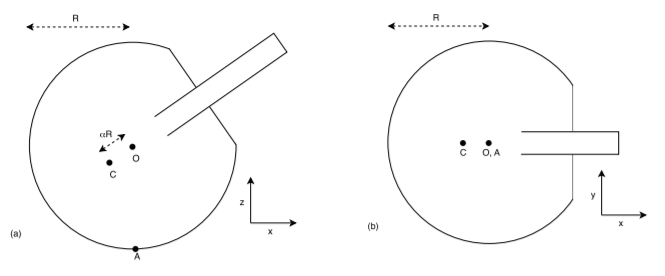
\includegraphics[width=\linewidth]{pictures/TIP_1}}
	\caption{ Вид на Tippe Top (а) сбоку и (б) сверху}
	\label{figimage1}
\end{figure}

\subsection{Описание поведения волчка }

Пусть $(x;y;z)$ -- вращающаяся система отсчета, определенная таким образом, что $\hat{z}$ неподвижна и направлена вверх, а вершина оси симметрии находится в плоскости $xy$. На $\textit{рисунке 1}$ показаны два вида на волчок Tippe Top: сбоку, и сверху. Как показано на Рисунке 1 (б), ось симметрии волчка совмещена с осью $x$, если смотреть сбоку. 

На рисунке 2 показано движение волчка на нескольких этапах после начала вращения:

(а) \textbf{фаза I}: сразу после ее первоначального запуска, при $\theta \sim 0$

(б) \textbf{фаза II}: вскоре после этого, наклонившись на угол $0 <\theta < \frac{\pi}{2}$

(в) \textbf{фаза III}: когда стержень впервые касается пола, при $\theta > \frac{\pi}{2}$

(г) \textbf{фаза IV}: после переворота, когда волчок вращается на своей ножке, с $\theta \sim \pi$ 

(д) \textbf{фаза V}: в конечном состоянии, покоющийся на стержне, при $\theta = \pi$

\begin{figure}[!ht]
	\center{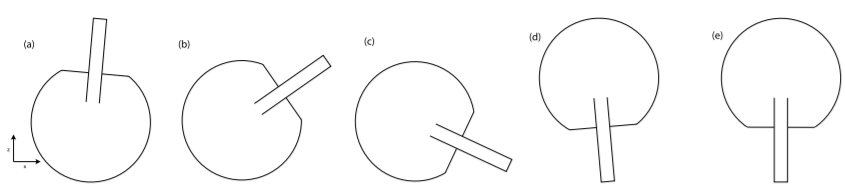
\includegraphics[width=\linewidth]{pictures/TIP_2}}
	\caption{ Фазы с I по V движения волчка Tippe Top, показанные в $xy$-				плоскости}
	\label{figimage2}
\end{figure}
%%%%
\vspace{1em}


\subsection{Описание новых систем координат}

При будущем исследовании поведения волчка для удобства нам понадобятся новые системы координат, поэтому введем новую систему отсчета: пусть $(X;Y;Z)$ - инерциальная система отсчета, у которой поверхность, на которой находится вершина, полностью лежит в плоскости $XY$. Система  отсчета $xyz$ определяется, как указано выше, и достигается из $XYZ$ посредством вращения вокруг оси $Z$ на угол $\phi$. Преобразование от системы отсчета $XYZ$ к системе отсчета $xyz$ показано на рисунке 3 (а). В частности, $\hat{z}$ = $\hat{Z}$.

\begin{figure}[h]
	\center{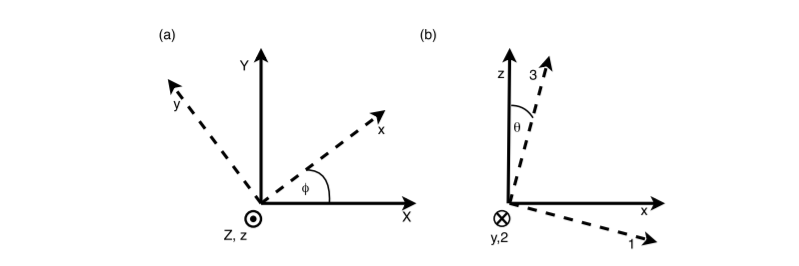
\includegraphics[width=\linewidth]{pictures/TIP_3}}
	\caption{ Преобразования между системами отсчета: (а) в $xyz$ из $XYZ$, и (б) из $xyz$ в 123}
	\label{figimage3}
\end{figure}


Любое вращательное движение в трехмерном пространстве можно описать тремя углами Эйлера ($\theta$, $\phi$, $\psi$). Преобразования между инерциальной системой отсчета $XYZ$, промежуточной системой отсчета $xyz$ и системой отсчета вершин $123$ можно объяснить в терминах этих углов Эйлера.

Небольшой экскурс : Сферическая система координат — трёхмерная система координат, в которой каждая точка пространства определяется тремя числами ${\displaystyle (r,\;\theta ,\;\varphi )}$, где ${\displaystyle r}$ -- расстояние до начала координат (радиальное расстояние), а ${\displaystyle \theta }$  и ${\displaystyle \varphi }$  -- зенитный и азимутальный углы соответственно. 

Понятия зенит и азимут широко используются в астрономии. Зенит -- направление вертикального подъёма над произвольно выбранной точкой (точкой наблюдения), принадлежащей фундаментальной плоскости. В качестве фундаментальной плоскости в астрономии может быть выбрана плоскость, в которой лежит экватор, или плоскость, в которой лежит горизонт, или плоскость эклиптики и т. д., что порождает разные системы небесных координат. Азимут -- угол между произвольно выбранным лучом фундаментальной плоскости с началом в точке наблюдения и другим лучом этой плоскости, имеющим общее начало с первым. Для простоты понятия приведем соответствующий рисунок, изображающий вышесказанное описание сферической системы координат.

\begin{figure}[h]
	\center{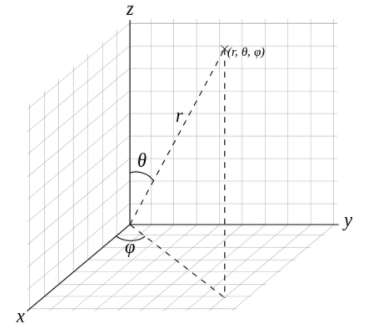
\includegraphics[scale = 0.75]{pictures/Angles}}
	\caption{Сферическая система координат наглядно}
	\label{Angles}
\end{figure}



В нашем описании движения волчка Tippe Top углы $\theta$ и $\phi$ являются стандартными зенитным и азимутальным углами соответственно в сферических полярных координатах. В системе координат $XYZ$ они определяются следующим образом: $\theta$ -- это угол оси симметрии волчка от вертикальной оси $Z$, показывающий, насколько далеко от вертикали его стержень есть, в то время как $\phi$ представляет угловое положение верха относительно оси $Z$ и определяется как угол между плоскостью $XY$ и плоскостью, проходящую через точки $O$, $A$, $C$ (т.е. вертикальная проекция симметрии волчка ось).

Третий угол Эйлера $\psi$ описывает вращение волчка вокруг собственной оси симметрии, то есть его <<спин>>, который имеет угловую скорость $\dot{\psi}$.

Система отсчета волчка определяется как новая вращающаяся система координат $(1;2;3)$, которая достигается путем поворота $xyz$ на $\theta$ вокруг $\hat{y}$: <<наклон>> оси $\hat{z}$ вниз нa $\theta$, чтобы соответствовать оси симметрии волчка ($\hat{3}$). Преобразование от системы координат $xyz$ в систему координат $123$ показано на рисунке 3 (b). В частности, $\hat{2}$ = $\hat{y}$.

Стоит сделать небольшое примечание:
Для системы отсчета $\mathbf{\stackrel{\sim}{\textbf{K}}}$, вращающейся в инерциальной системе $\textbf{K}$ с угловой скоростью $\mathbf{\omega}$, производные по времени вектора $\textbf{A}$ в обеих системах $\textbf{K}$ и $\mathbf{\stackrel{\sim}{\textbf{K}}}$ связаны соотношением:

\begin{equation}
\boxed{
	\left(\frac{\partial \textbf{A}}{\partial t}\right)_{\textbf{K}} = \left( 			\frac{\partial \textbf{A}}{\partial t} \right)_{\mathbf{\stackrel{\sim}				{\textbf{K}}}} + \left[\mathbf{\overrightarrow{\omega}}\times \mathbf{\overrightarrow{A}}\right]
	}
	\label{eq1} 
\end{equation}

Движение волчка Tippe Top является сложным и включает в себя изменение со временем трех углов Эйлера, а также поступательной скорости (или положения) и движение оси симметрии волчка. Все эти параметры связаны. Чтобы определить движение волчка Tippe Top, можно использовать стандартные инструменты, включая Законы Ньютона для составления систем уравнений, а затем программирование компьютера для их численного решения с помощью моделирования.

Этим вопросом мы и будем заниматься в этой работе, исследуя физику волчка Tippe Top, чтобы составить систему уравнений. А в [заключении] исследуем полученные результаты.

Трение между волчком Tippe Top и поверхностью, по которой он движется, приводит в движение волчок. Предполагается, что верхняя часть остается в контакте с поверхностью в точке $A$ до тех пор, пока стержень не коснется поверхности. Он движется в точке $A$ со скоростью $v_A$ относительно поверхности. Коэффициент трения $\mu_k$ между верхушкой и поверхностью, возникающий в результате движения, с $|\overrightarrow{F_f}|$ = $\mu_kN$, где $\overrightarrow{F_f}$ = $F_{f,x} \hat{x}$ + $F_{f,y} \hat{y}$ -- сила трения, а $F_{f,x} \hat{x}$ и $F_{f,y} \hat{y}$ -- это его проекции на оси $x$ и $y$ соответственно, $N$ -- величина нормальной силы. Предположим, что волчок изначально настроен только на вращение, т.е. нет поступательного импульса на волчок.

Пусть масса волчка Tippe Top равна $m$. Его моменты инерции: $I_3$ относительно оси симметрии, а $I_1 = I_2$ относительно взаимно перпендикулярных главных осей. Пусть $\vec{s}$ -- вектор положения центра
масса, а $\vec{a} = \overrightarrow{CA}$ -- вектор от центра масс к точке контакта.

\begin{center}
	\section{Подробное описание поведения волчка}
\end{center}

В данном разделе займемся уже более интересными вещами, а именно подробно опишим модель поведения волчка Tippe Top на плоскости при наличии силы трения.

Так же для простоты и краткости скалярное произведение векторов $\vec{a}$ и $\vec{b}$ будем обозначать просто как $\vec{a}\cdot \vec{b}$, а в тех местах, где не нужно скалярное произведение векторов, знак "$\cdot$"\textbf{ }будем опускать.

\subsection{Небольшое вступление в теорию описания}
Так как при наличии некоторых данных о связи двух систем координат между собой мы умеем переходить от одной системы координат в другую, тогда выразим переход от системы координат $XYZ$ в систему координат $xyz$:

\begin{equation}
	\begin{pmatrix}
		\hat{x} \\
		\hat{y} \\
		\hat{z} 
	\end{pmatrix}
	= 
	\begin{pmatrix}
		\cos\phi & \sin\phi & 0\\
		-\sin\phi & \cos\phi & 0\\
		0 & 0 & 1
	\end{pmatrix}
	\begin{pmatrix}
		\hat{X} \\
		\hat{Y} \\
		\hat{Z} 
	\end{pmatrix}
	\label{eq2}
\end{equation}\\
Аналогичным образом выразим переход в систему координат $123$ от $xyz$:

\begin{equation}
	\begin{pmatrix}
		\hat{1} \\
		\hat{2} \\
		\hat{3} 
	\end{pmatrix}
		= 
	\begin{pmatrix}
		\cos\theta & 0 & -\sin\theta\\
		0 & 1 & 0\\
		\sin\theta & 0 & \cos\theta
	\end{pmatrix}
	\begin{pmatrix}
		\hat{x} \\
		\hat{y} \\
		\hat{z} 
	\end{pmatrix}
	\label{eq3}
\end{equation}\\
Положение точки $A$ от центра масс в системах координат $xyz$ и $123$:

\begin{equation}
\boxed{
\vec{a} = \alpha R \hat{3} - R\hat{z} 
  = \alpha R \theta \hat{x} + R(\alpha \cos\theta - 1)\hat{z}
  = R \sin\theta \hat{1} + R(\alpha - \cos\theta)\hat{3}
}
	\label{eq4}
\end{equation}\\
%%%%%%%%%%
\newpage
Так же можно получить полезное соотношение,  которое нам понадобится в будущем:

\begin{equation}
\boxed{
	\left[\hat{z}\times \hat{3}\right] = \hat{y} \sin\theta 
}
	\label{eq5}
\end{equation}

Так же нам понадобится одно замечание, данное выше, уравнение (\ref{eq1}).

Производные, необходимые нам в дальнейшем, координат по времени:

\begin{equation}
\boxed{
	\dot{\hat{3}} = \left[\omega \times \hat{3}\right]
}
	\label{eq6}
\end{equation}

\begin{equation}
	\dot{\hat{x}} = \phi \hat{y}
	\label{eq7}
\end{equation}

\begin{equation}
	\dot{\hat{y}} = -\phi \hat{x}
	\label{eq8}
\end{equation}

\subsection{Поиск внешних сил}

Диаграмма свободного тела, с изображенными силами, действующими на него:

\begin{figure}[h]
	\center{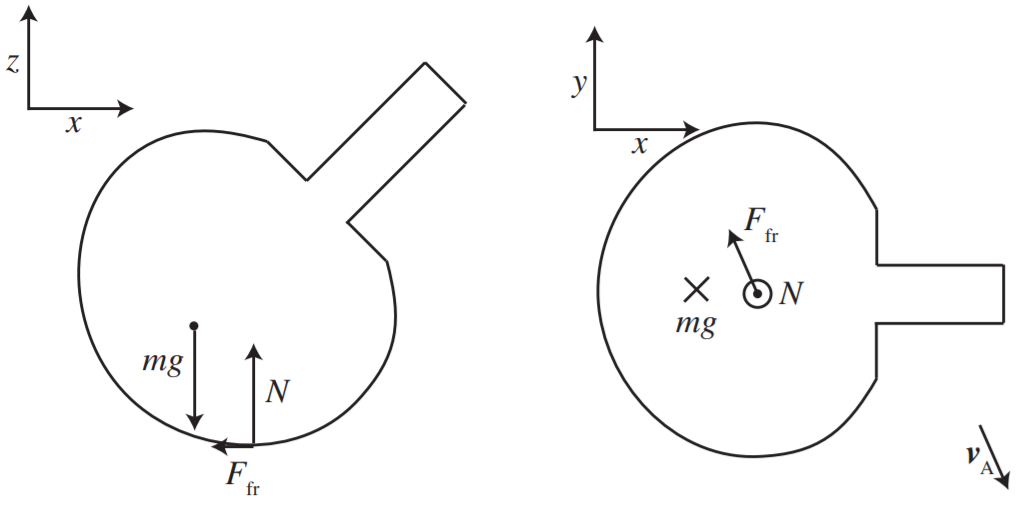
\includegraphics[width=\linewidth]{pictures/TIP_4}}
	\caption{}
	\label{figimage5}
\end{figure}

Примечание: направление $\overrightarrow{F_f}$ должно быть противоположным направлению $\overrightarrow{v_A}$. Сумма сил:
%%%%%%%%%%%%%%%%
\begin{equation}
	\overrightarrow{F_{ext}} = (\overrightarrow{N} - \overrightarrow{mg})\cdot \hat{z} + \overrightarrow{F_f} = (\overrightarrow{N} - \overrightarrow{mg})\cdot \hat{z} - \frac{\mu_k N}{|v_A|}\overrightarrow{v_A}
	\label{eq9}
\end{equation}

\subsection{Поиск общего внешнего крутящего момента $\tau_{ext}$ на вершите Tippe Top'a относительно центра масс}
%%%%%%%%%%%%%%%%%%%%
Сумма крутящих моментов:

\begingroup
\everymath{\scriptstyle}
\scriptsize
\begin{equation}
\boxed{
	\overrightarrow{\tau_{ext}} = \left[\vec{a} \times (N\hat{z}+ \overrightarrow{F_f})\right] = \left[(\alpha R \hat{3}) \times (N \hat{z} + 	F_{f,x}\hat{x} + F_{f,y}\hat{y})\right]
}
	\label{eq10}
\end{equation}
%%%%%%
	\[
	 = [\alpha R N \hat{3}  \times \hat{z}] + \left[\alpha R (\sin\theta \hat{x} + \cos \theta \hat{z})\times(F_{f,x}\hat{x} + F_{f,y}\hat{y})\right] - \left[R \hat{z} \times 			(F_{f,x}\hat{x} + F_{f,y}\hat{y})\right]
	\]
	\[
 	= -\alpha R N \sin\theta \hat{y} + \alpha R \sin\theta F_{f,y} \hat{z} + 			\alpha R \cos\theta F_{f,x} \hat{y}-\alpha R \cos\theta F_{f,y}\hat{x} - 			RF_{f,x}\hat{x} - RF_{f,x}\hat{x} +RF_{f,x}\hat{x}
	\]
%%%%%%
	\begin{equation}
		=RF_{f,y}(1 - \alpha \cos\theta)\hat{x}  + \left[RF_{f,x}(\alpha \cos\theta - 			1)- \alpha RN\sin\theta \right] \hat{y} + \alpha R \sin\theta F_{f,y}\hat{z}
		\label{eq11}
	\end{equation}
\endgroup


\subsection{Движение в точке касания ($A$)}
%%%%%%%%%
Движение в точке $A$ удовлетворяет следующему уравнению:

\begin{equation}
\boxed{
	\overrightarrow{v_a} =\dot{\vec{s}} + \left[\overrightarrow{\omega} \times \vec{a}\right]
}
	\label{eq12}
\end{equation}

где $\omega$ - полная угловая скорость волчка в системе центра масс (это определяется в следующая часть). Хочу показать, что $\overrightarrow{v_A} \cdot \hat{z}$ = 0.

Чтобы показать это, возьмем производную по времени от условия контакта в системе координат $XYZ$ или $xyz$ (примечание: подходит любой вариант, поскольку нам нужна только компонента $\hat{z}$, а $\hat{z} = \hat{Z}$).

Условия контакта:
\begin{multline}
	(\vec{s} + \vec{a})\cdot \hat{z} = 0 \hspace{25.5mm} \text{ всегда, то есть в любой момент 	времени}\\
	\Rightarrow \frac{d}{dt}(\vec{s} + \vec{a})\cdot \hat{z} = 0\hspace{5mm} \text{ аналогично в 	любой момент времени}
	\label{eq13}
\end{multline}

Обратим внимание, что нас интересует только $z$--компонента, и ($\omega \times \hat{z}) \cdot \hat{z} = 0$. Тогда, используя (\ref{eq12}), (\ref{eq4}) и (\ref{eq5}) получаем:

\begin{multline}
	\\
	\overrightarrow{v_A} \cdot \hat{z} = (\dot{\vec{s}} + [\overrightarrow{\omega} \times \vec{a}])\cdot \hat{z}\\
	= (\dot{\vec{s}} + [(\alpha R \overrightarrow{\omega}) \times \hat{3}])\cdot \hat{z}
	\\
	= (\dot{\vec{s}} + \alpha R \frac{d\hat{3}}{dt})\cdot \hat{z}
	\\
	=(\dot{\vec{s}}+ \dot{\vec{a}})\cdot \hat{z} = 0\\
	\label{eq14}
\end{multline}

\subsection{Угловая скорость $\omega$ вращающегося волчка относительно его центра масс $C$}

Найдем полную угловая скорость $\omega$ вращающегося волчка относительно его центра масс $C$ через производные по времени от углов Эйлера: $\dot{\theta} = \frac{d\theta}{dt}, \dot{\phi} = \frac{d\phi}{dt},\dot{\psi} = \frac{d\psi}{dt}.$

Общая угловая скорость волчка $\omega$ складывается из трех различных вращений.

\begin{equation}
	\overrightarrow{\omega} = \dot{\theta}\hat{2} + \dot{\phi}\hat{z} + \dot{\psi} \hat{3}
	\label{eq15}
\end{equation}

Используем преобразования, показанные на рисунке 3, чтобы преобразовать в систему координат $xyz$ или $123$:

\begin{equation}
	\overrightarrow{\omega} = \dot{\psi}\sin\theta \hat{x} + \dot{\theta} \hat{y} + (\dot{\psi}\cos 	\theta + \dot{\phi})\hat{z}
	\label{eq16}
\end{equation}

\begin{equation}
\boxed{
	\overrightarrow{\omega} = -\dot{\phi}\sin \theta\hat{1} + \dot{\theta}\hat{2} + (\dot{\psi}+			\dot{\phi}\cos\theta)\hat{3}
}
	\label{eq17}
\end{equation}


\subsection{Полная энергия вращения волчка}

Найдем полную энергию вращающегося волчка в терминах производных по времени от углов Эйлера, $u_x$, и $u_y$.

$\textbf{I}$ -- тензор инерции:

\begin{equation}
	\begin{pmatrix}
		I_1 & 0 & 0\\
		0 & I_2 & 0\\
		0 & 0 & I_3
	\end{pmatrix}
	\label{eq18}
\end{equation}

Стоит отметить, что $I_2 = I_1$ в силлу симметрии нашего тела (будем в дальнейшем обозначать $I_2$ как $I_1$). Таким образом имеем 
\begin{equation}
	E_T = K_T + K_R + U_G = \frac{1}{2}(\overrightarrow{\omega} \cdot \textbf{I}\overrightarrow{\omega}) + \frac{1}{2}m\dot{s}^2 	+ mgR(1 - \alpha \cos\theta)
	\label{eq19}
\end{equation}

Пользуясь уравнением (\ref{eq12}) получим следующее:

\begin{multline}
	\\
	\dot{\vec{s}} = \overrightarrow{v_A} - \left[\overrightarrow{\omega} \times \vec{a}\right]
	\\
	= \overrightarrow{v_a} - \left[(\dot{\theta}\hat{2} + \dot{\phi}\hat{z} + \dot{\psi}\hat{3})\times(\alpha R \hat{3} - R\hat{z})\right]
	\\
	= u_x\hat{x} + u_y\hat{y} - (\dot{\theta}\alpha R \hat{1} - \dot{\theta}R\hat{z} + \left[\dot{\phi}\alpha R \hat{z} \times \hat{3}\right] - \left[\dot{\psi} R \hat{3} \times \hat{z}\right])
	\\
	= (u_x + \dot{\theta}R(1 - \alpha \cos \theta))\hat{x} + (u_y - R\sin \theta(\alpha \dot{\phi} + \dot{\psi}))\hat{y} + \dot{\theta}\alpha R \sin \theta 		\hat{z}
	\label{eq20}
\end{multline}

Таким образом, используя уравнение (\ref{eq5}), получаем:

\begin{multline}
	\\
	E_T = \frac{1}{2}\left[ I_1(\dot{\phi}^2\sin^2\theta + \dot{\theta}^2) + 			I_3(\dot{\psi} + \dot{\phi}\cos \theta)^2 \right] +
	\\
+ \frac{m}{2}\left[ \left(u_x + \dot{\theta}R(1 - \alpha\cos \theta)\right)^2 + \left(u_y - R\sin\theta (\alpha \dot{\phi} + \dot{\psi})\right)^2 + \dot{\theta}^2\alpha^2R^2\sin^2\theta \right] + 
\\
+ mgR(1 - \alpha\cos \theta)
	\label{eq21}
\end{multline}

\subsection{Изменение момента импулься относительно оси $z$}

Из (\ref{eq10}) уравнения получаем:

\begin{equation}
\boxed{
	\frac{d\vec{L}}{dt}\cdot \hat{z} = \sum\overrightarrow{\tau} \cdot \hat{z} = \alpha R \sin 	\theta F_{f,y}
}
	\label{eq22}
\end{equation}

\subsection{Выражение для мгновенной скорости изменения энергии волчка}

Изменения в энергии: так как  $h = \vec{s} \cdot \hat{z}$ увеличивается, поэтому $\dot{U_G} > 0$.

В начале и в конце (фазы \textbf{I} и \textbf{V}) есть небольшая трансляция, поэтому $K_T \sim 0$ в \textbf{I} и \textbf{V}. Таким образом, энергия переводится из $K_R$ в $U_G$.

Нормальная сила не работает, то есть не вносит вклад в работу. В точке $A$ работает сила трения, а направление $-v_A$:

\begin{equation}
	W = \int \overrightarrow{F_f} \cdot \overrightarrow{v_A} dt < 0 \ \Rightarrow \ \frac{d}{dt}E_T = -\mu_k N|\overrightarrow{v_A}|
	\label{eq23}
\end{equation}

Таким образом мы определили, что $\overrightarrow{F_f}$ монотонно уменьшает полную энергию.

(\ref{eq22}) уравнение подразумевает, что только $\overrightarrow{F_f} \cdot \hat{y}$ уменьшает $\overrightarrow{L}\cdot \hat{z}$. Передача энергии от $K_R$ к $U_G$, вызванная составляющей силы трения в направлении $\hat{y}$, поэтому составляющая результирующего крутящего момента находится в направлении результирующего вектора [$\vec{a}\times \hat{y}$].


\subsection{Построение и анализ графиков функций энергий от времени}

Теперь уже мы можем качественно изобразить следующие энергетические термины  как функцию времени движения волчка в пяти фазах (\textbf{I} -- \textbf{V}) , показанных на рисунке (\ref{figimage2}):
%%%%%%
\begin{enumerate}
	\item Полная энергия $E_T$.
	\item Гравитационная потенциальная энергия $U_G$.
	\item Поступательная кинетическая энергия $K_T$.
	\item Кинетическая энергия вращения $K_R$.
\end{enumerate}


\newpage
\begin{figure}[h!]
	\center{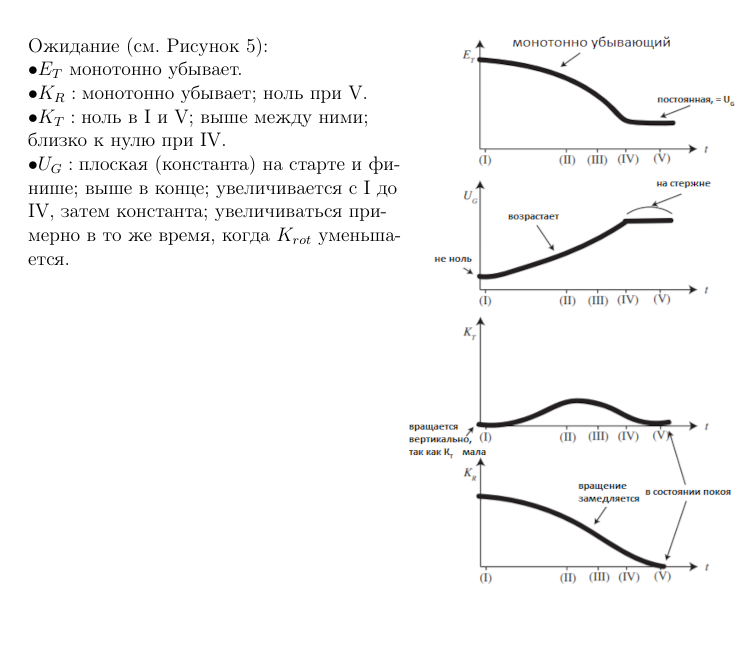
\includegraphics[scale = 0.7707135]{pictures/TIP_5}}
	\label{figimage6}
\end{figure}


\subsection{Связь компонентов углового момента $L$ и угловой скорости $\omega$}
%%%%
Покажем, что компоненты углового момента $L$ и угловой скорости $\omega$, которые перпендикулярны направлению вектора $\hat{3}$, пропорциональны и выполняется:

\begin{equation}
	[\vec{L} \times \hat{3}] = k\left[\overrightarrow{\omega} \times \hat{3}\right],
	\label{eq24}
\end{equation}
%%%%%%
Так же найдем этот коэффициент пропорциональности.\\
Из соотношения (\ref{eq17}):

\begin{equation}
	\vec{L} = \textbf{I}\overrightarrow{\omega} = I_1(-\dot{\phi}\sin \theta \hat{1} + \dot{\theta}\hat{2}) + I_3(\dot{\psi} + \dot{\phi}\cos \theta)\hat{3}
	\label{eq25}
\end{equation}
Возьмем векторное произведение обоих частей с $\hat{3}$:

\begin{equation}
\boxed{
	\left[\vec{L}\times \hat{3}\right] = I_1(\dot{\phi}\sin \theta \hat{2} + \dot{\theta} \hat{1}) = I_1 \left[\overrightarrow{\omega} \times \hat{3}\right]
}
	\label{eq26}
\end{equation}

\subsection{Интеграл Джеллетта}

Объединение полученных результатов дает нам следующие:
\begin{enumerate}
	\item Величину $N$ нормальной силы.
	\item Системы уравнений, связывающих углы Эйлера, компоненты $u_x$ и $u_y$ скорости 	в точке $A$, единичный вектор для оси симметрии $\hat{3}$, и их производные по 			времени.
\end{enumerate}

Эта система не интегрируема, то вместо этого может быть решена численно. 

Интегралы движени -- это величины, которые остаются постоянными и могут уменьшить размерность системы (то есть количество одновременных уравнений, которые необходимо решить, аналитически или численно). Обычно такие величины, как энергия, импульс и угловой момент, сохраняются в закрытых системах, и значительно упрощают задачу.

Как мы увидели, ни энергия, ни угловой момент не сохраняются для Tippe Top --  из-за рассеивающей силы и внешнего крутящего момента. Однако есть
связанная величина, известная как интеграл Джеллетта $\lambda$, которая представляет собой компонент, который сохраняет угловой момент, т.е. некоторый вектор $v$. такой, что $\lambda$ = $\vec{L}\cdot \vec{v}$ постоянна во времени.

Используем наше понимание Tippi Tip и полученный результаты, чтобы дать выражение для такого вектора $v$. Так же покажем, что производная по времени равна нулю, то есть $\lambda$ постоянна во времени.

Для любой оси, проходящей через центр масс справедливо следующее:

\begin{equation}
	\frac{d\vec{L}}{dt} \neq 0 \Leftrightarrow \overrightarrow{\tau_{ext}} \neq 0
	\label{eq27}
\end{equation}

Внешний крутящий момент получим из (\ref{eq10}):

\begin{equation}
	\overrightarrow{\tau_{ext}} = \left[\vec{a} \times (N\hat{z} + \vec{F_f})\right] \Rightarrow \overrightarrow{\tau_{ext}}\cdot \vec{a} = 0
	\label{eq28}
\end{equation}
%%%%%
\begin{equation}
	\frac{d\vec{L}}{dt}\cdot \vec{a} = 0
	\label{eq29}
\end{equation}

Таким образом, угловой момент в направлении $\vec{a}$ должен быть постоянным, поэтому $\vec{v} = \vec{a}$.

Продемонстрировать это математически позволяют уравнения (\ref{eq6}), (\ref{eq10}), (\ref{eq26}):
\begin{multline}
\\
-\dot{\lambda} = \frac{d\vec{L}}{dt}\cdot \vec{a} + \alpha R\vec{L}\cdot \frac{d\hat{3}}{dt} = \left[\vec{a}\times (N\hat{z} + \overrightarrow{F_f})\right]\cdot \vec{a} + \frac{\alpha R}{I_1}\vec{L}\cdot \left[\overrightarrow{\omega} \times \vec{L}\right] = 0
	\label{eq30}
\end{multline}

\section{Заключение}

Изучена поставленная нами задача о движении волчка Tippe Top на плоскости с
трением. Рассмотрена модель сферического волчка.


\section{Список используемой литературы}

$\bullet$ Ландау Л. Д., Лифшиц Е. М. Механика. — 5-е изд., стереотип. — М.: ФИЗМАТЛИТ, 2012. — 224 с. — 500 экз. — ISBN 978-5-9221-0819-5\\
\\
$\bullet$ Курс аналитической геометрии и линейной алгебры: [учеб. для вузов]\\
\\
$\bullet$ Зобова А.А., Карапетян А.В. Анализ стационарных движений волчка тип-топ // ПММ. 2009. Т. 73,
№ 6. C. 867-877\\
\\ 
$\bullet$ \href{https://en.wikipedia.org/wiki/Tippe_top}{[EN] Wiki (Tippe Top)}\\
\\
$\bullet$ \href{https://ru.wikipedia.org/wiki/\%D0\%9A\%D0\%B8\%D1\%82\%D0\%B0\%D0\%B9\%D1\%81\%D0\%BA\%D0\%B8\%D0\%B9_\%D0\%B2\%D0\%BE\%D0\%BB\%D1\%87\%D0\%BE\%D0\%BA}{[RU] Wiki (Китайский волчок)}

					\end{document}
